\chapter{Desafios de segurança de CDN}
\label{sec:seguranca}
 Podemos definir seguran\c{c}a como um conjunto de a\c{c}\~oes que e dos recursos utilizados para proteger algo ou algu\'em, ou, o que serve para diminuir os riscos ou perigo. Portanto, seguran\c{c}a \'e um tema extramente abrangente e complexo. Podemos falar de t\'opicos como seguran\c{c}a f\'isica, social, de um sistema ou at\'e mesmo de um grupo de servidores interconectados, que \'e o caso da CDN, e ainda coloca-los todos dentro do mesmo grupo. Ou seja, podemos trat\'a-los de forma separada ou analisando o conjunto todo.
 
Ainda dentro de Seguran\c{c}a de CDN podemos tratar de pontos principais, onde o vazamento \'e ponto crucial e mais l\'ogico de ser atacado. 
\begin{figure}[H]
\caption{Objetivos da seguran\c{c}a}
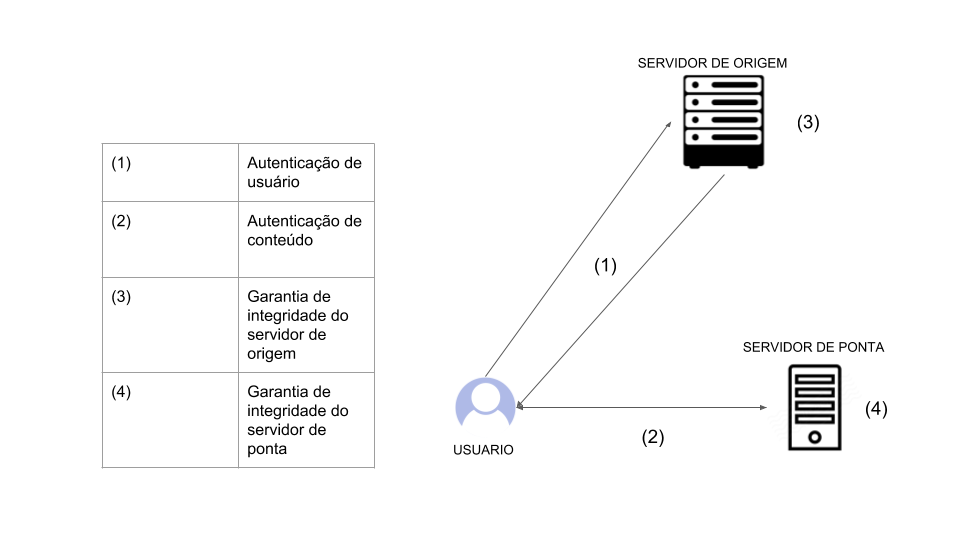
\includegraphics[height=9cm]{Figuras/seguranca_intro.png} 
\label{figura:seguranca_intro}
\end{figure}

Como vemos na figura \ref{figura:seguranca_intro} podemos observar que se tem quatro grandes pontos a serem garantidos em uma rede. Dois deles (1) e (2) de autentica\c{c}\~ao e outros dois (3) e (4) relacionados a integridade. O primeiro trata-se da autentica\c{c}\~ao de usu\'ario que \'e capacidade do sistema de garantir que aquele usu\'ario que est\'a acessando o conte\'udo tem mesmo os requisitos para acess\'a-lo. Ou seja, \'e mesmo um usu\'ario do sistema. Por ser um tema bem abrangente ser\'a tratado com mais profundidade em \ref{subsection:autenticacao_usuario}.

Em segundo lugar temos a autentica\c{c}\~ao de conte\'udo. Que \'e a garantia que o conte\'udo acessado \'e o mesmo buscado pelo usu\'ario, que o usu\'ario tem acesso a ele e tamb\'em \'e um conte\'udo que faz parte da rede de disponibilidade da CDN(que n\~ao \'e um conte\'udo inserido por terceiro sem autoriza\c{c}\~ao pr\'evia). Tudo isso tem que ser minuciosamente tratado e averiguado antes de retornar ao usu\'ario. Tudo isso ser\'a abordado em \ref{subsection:autenticacao_conteudo}.

Nos dois outros, (3) e (4), trata-se da seguran\c{c}a dos servidores. A\'i podemos falar de seguran\c{c}a f\'isica e l\'ogica. Tem-se que levar em conta a forma de acesso de cada um na hora de mensurar os aspectos de seguran\c{c}a de cada um deles. 

No servidor de origem se tem um acesso via HTTP, com um endereço "leg\'ivel". Esse acesso se dar\'a muitas vezes por v\'arias parte do globo, tendo que deix\'a-lo dispon\'ivel , portanto, vulner\'avel \`a diversos tipos de ataque, o que o torna extremamente complexo na hora de definir suas regras de seguran\c{c}a, n\~ao basta apenas subir um \textit{firewall} bloqueando m\'ultiplos acessos, \'e preciso saber exatamente os tipos de aplica\c{c}\~oes que ser\~ao tratadas para assim come\c{c}ar a desenhar as regras de \textit{firewall} que ser\~ao aplicadas.

J\'a no servidor de ponta a preocupa\c{c}\~ao com o acesso via HTTP j\'a \'e uma coisa a menos, visto que muitas vezes o acesso funcionar\'a via redirecionamento do servidor de origem, sendo o controle de endere\c{c}o feito pelo o mesmo. Mas h\'a diversos outros aspectos que tem que serem levados em conta, como parte da autentica\c{c}\~ao de conte\'udo para o usu\'ario, que nada mais \'e que garantir que o usu\'ario para o qual est\'a sendo enviado o conte\'udo tem acesso ao mesmo. Outra grande preocupa\c{c}\~ao \'e quanto a sua disponibilidade, pois \'e necess\'ario que o mesmo esteja "de p\'e" quando for requisitado conte\'udo e que durante o processo de transfer\^encia, caso haja alguma interrup\c{c}\~ao a mesma seja informada ao servidor de origem e o usu\'ario transferido para outro servidor sem que haja muitos danos \`a experi\^encia. Isso sem contar nas enumeras preocupa\c{c}\~oes que se deve ter com servidores. No livro \cite{stallings1995network} se pode aprofundar um pouco mais nessas quest\~oes de segurança na \textit{web}.

Mas para se aprofundar um pouco mais dentro dos conceitos de seguran\c{c}a de usu\'ario e conte\'udo de uma CDN \'e necess\'ario primeiro conhecer um pouco sobre protocolos AAA que ser\'a tratado em \ref{subsection:AAA}.
\section{protocolos AAA - Authentication, Authorization, and Accounting}
\label{subsection:AAA}
A associa\c{c}\~ao dos protocolos de autentica\c{c}\~ao, autoriza\c{c}\~ao e auditoria em um termo, protocolos AAA, se deu porque na maioria dos sistemas seguros esses tr\^es protocolos s\~ao extremamente necess\'arios e amplamente utilizados. em \cite{metz1999aaa} se pode aprofundar melhor. Mas vamos h\'a uma r\'apida s\'intese dos mesmos.
\paragraph{Autentica\c{c}\~ao}- Verifica a identidade digital do usu\'ario de um sistema, que segundo \cite{metz1999aaa}, envolve a valida\c{c}\~ao da identidade do usu\'ario final afim de permitir seu acesso \`a rede.

Esse procedimento \'e baseado na apresenta\c{c}\~ao de uma identidade junto com uma ou mais credenciais, que podem ser senhas, certificados digitais e etc.
\paragraph{Autoriza\c{c}\~ao}- \'E a concess\~ao de uso para determinados servi\c{c}os. Essa etapa s\'o \'e acionada mediante a autentica\c{c}\~ao pr\'evia de um usu\'ario. Ela leva em conta a identidade, o servi\c{c}o requerido e o estado atual do sistema. Muitas vezes ela trabalha com a utiliza\c{c}\~ao de filtros para retornar que tipo de protocolos ou aplica\c{c}\~oes s\~ao suportadas.

Na maioria dos casos os protocolos de autentica\c{c}\~ao e autoriza\c{c}\~ao trabalham juntos. Onde um depende diretamente do funcionamento do primeiro. Em ambientes de VOD, como se foi apresentado em \ref{subsubsection:vod_exemplo}, essa etapa normalmente \'e verificada nos servidores de ponta, os quais s\~ao respons\'aveis por fornecer o conte\'udo ao usu\'ario.
\paragraph{Auditoria}- A \'utima etapa do processo \'e relacionada a coleta de informa\c{c}\~oes de tr\'afego utilizado pelo usu\'ario. 

H\'a dois tipos de coletas: coletas em tempo real e coleta \textit{batch}. A primeira se refere a informa\c{c}\~oes captadas em tempo de uso, ou seja, enquanto o usu\'ario faz uso da rede essas informa\c{c}\~oes s\~ao enviadas. J\'a a segunda se refere a uma coleta que \'e primeiro armazenada e enviadas posteriormente. 

S\~ao essas informa\c{c}\~oes que s\~ao utilizadas pelas operadoras para cobran\c{c}a e taxa\c{c}\~ao do servi\c{c}os de VOD.
\section{Autentica\c{c}\~ao de usu\'ario}
\label{subsection:autenticacao_usuario}
A autentica\c{c}\~ao de usu\'ario envolve a a certeza que o usu\'ario que est\'a consumindo o conte\'udo ou tentando acessar a rede \'e o mesmo usu\'ario que tem acesso \`a aplica\c{c}\~ao. E o que acontece quando o usu\'ario faz login somente uma vez (em uma p\'agina)? Como garantir que \'e o mesmo usu\'ario?

Bom, a forma de armazenamento vai depender muito de onde est\'a sendo acessada a aplica\c{c}\~ao. Se for de um desktop, dentro de um navegador, normalmente vai ser armazenada dentro do \textit{cookies} do navegador. Se for de uma aplica\c{c}\~ao mobile, ou at\'e mesmo de uma aplica\c{c}\~ao desktop (sem ser um navegador), normalmente fica em alguma pasta tempor\'aria que \'e guardada pela mem\'oria \textit{flash}. Ent\~ao significa que uma vez feito login ele fica pra sempre armazenado?

N\~ao. Essas autentica\c{c}\~ao s\~ao tempor\'arias, muitas vezes com tempo de expira\c{c}\~ao definido pelas pr\'oprias aplica\c{c}\~oes, e requerem renova\c{c}\~ao da licen\c{c}a ou reautentica\c{c}\~ao do usu\'ario. 

Em todos os casos, h\'a diversas formas de autentica\c{c}\~ao dentro de sistemas computacionais. H\'a autentica\c{c}\~ao por login (normalmente email) e senha, por biometria, \textit{token} entre outras. Mas em aplica\c{c}\~oes \textit{web} login/senha s\~ao as mais utilizadas.

As etapas de verifica\c{c}\~ao de quantidade de aparelhos e a origem dos IPs de requisi\c{c}\~ao normalmente s\~ao feitas aqui.

Nesse processo \'e importante salientar tamb\'em a autentica\c{c}\~ao dos \textit{devices}. Nesse processo \'e muito importante que os \textit{devices} sejam limitados para que n\~ao haja vazamento de usu\'arios utilizando m\'ultiplas sess\~oes em mais de um dispositivo, quebrando assim a regra de que os acessos dos usu\'arios n\~ao podem serem compartilhados.

Na figura \ref{figura:autenticacao_conteudo} podemos v\^e quais processos, dentro do \textit{browser} , se comunicam com quais servidores.
\begin{figure}[H]
\caption{Comunica\c{c}\~ao: Processos x Servidores}
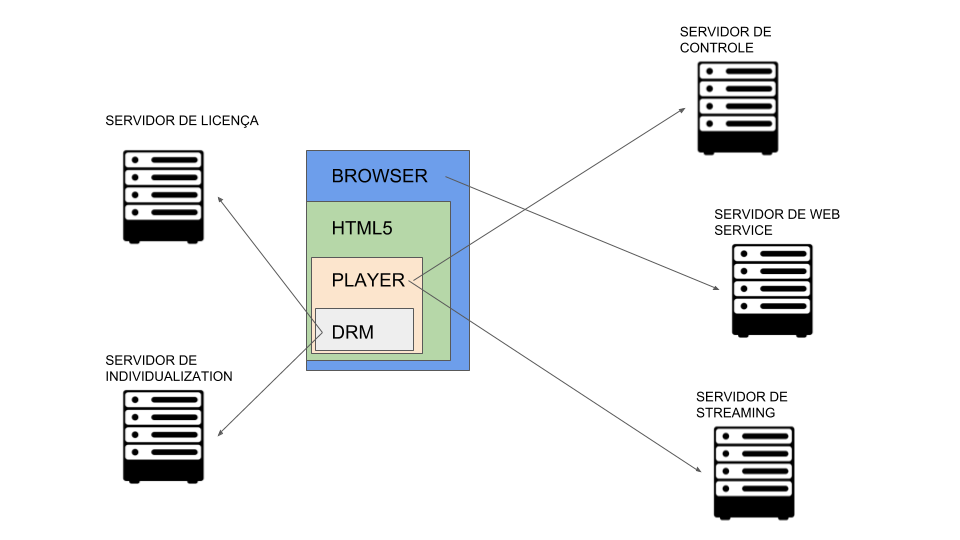
\includegraphics[width=14cm]{Figuras/autenticacao_conteudo.png} 
\label{figura:autenticacao_conteudo}
\end{figure}
\section{Certifica\c{c}\~ao de licen\c{c}as de conte\'udo}
\label{subsection:autenticacao_conteudo}
Dentro de certifica\c{c}\~ao de licen\c{c}as de conte\'udo h\'a uma gama de valida\c{c}\~oes que s\~ao ou que podem ser utilizadas, \cite{wein2012content} e \cite{leighton2007html} s\~ao duas delas.

Aqui iremos focar em uma chamada \textit{control DRM-encoded}, que \'e o m\'etodo mais utilizado hoje em dia. Utilizado inclusive por sistemas como Netfilx e VOD de operadoras de TV.

Esse processo est\'a intrinsecamente ligado ao processo de autentica\c{c}\~ao de usu\'ario explicado anteriormente. Nele o conte\'udo passa por uma s\'erie de valida\c{c}\~oes antes de tocar.

A primeira etapa do processo para tocar o conte\'udo \'e a etapa de \textbf{\textit{License Acquisition}}. Nela, apresentado por \cite{pomelo2009analysis}, antes de tocar \'e feito:
\begin{itemize}
\item Passo 1 -  A aplica\c{c}\~ao requisita do servidor um peda\c{c}o do conte\'udo. Este o retorna com o conte\'udo criptografado.
\item Passo 2 - O cliente l\^e o cabe\c{c}alho do conte\'udo criptografado e determina que aquele conte\'udo \'e criptografado. Para descriptografar o conte\'udo \'e necess\'ario que este tenha recebido a chave do servidor de licen\c{c}a. Caso n\~ao tenha recebido ele envia uma requisi\c{c}\~ao para adquiri-la. Se for a primeira vez que \'e feita a valida\c{c}\~ao da chave ele passa por um processo de \textit{individualization}. Que ser\'a explicado logo mais a frente.(figura \ref{figura:individualization}).
\item Passo 3 - O cliente recebe a licen\c{c}a do servidor, que antes de enviar a chave faz todo o processo de autencidade necess\'ario.
\item Passo 4 - O cliente ap\'os receber a chave pode tocar o conte\'udo. Isso se ele estiver licen\c{c}a para tal, \'e claro.
\end{itemize}

No passo 1 fica claro entender quando em \ref{subsec:vod} explicamos como \'e composto um VOD e qual o seu fluxo de comportamento.

O disparo do fluxo do \textit{individualization} \'e feito pela pr\'opia aplica\c{c}\~ao do cliente, que verifica caso o cliente n\~ao possua nenhuma licen\c{c}a ele aponta para um terceiro servidor, onde esse vai retornar com uma licen\c{c}a individual que ser\'a utilizada na hora de validar e tocar conte\'udo. O fluxo do processo \'e apresentado na figura \ref{figura:individualization}. 

Todo esse processo de troca de informa\c{c}\~oes \'e feito utilizando trocas de chaves assim\'etricas p\'ublicas garantindo assim a seguran\c{c}a e proced\^encia da informa\c{c}\~ao.
\begin{figure}[H]
\caption{autenticacao conte\'udo - \textit{individualization}}
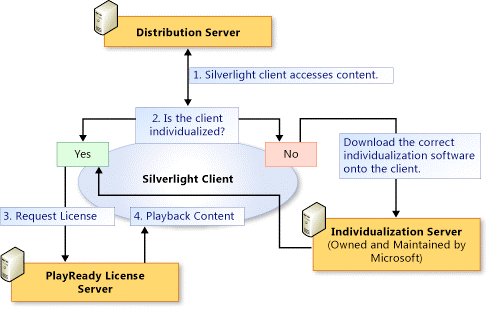
\includegraphics[height=9cm]{Figuras/autenticacao_conteudo_individualization.png} 
\label{figura:individualization}
\end{figure}
Ap\'os \textbf{\textit{License Acquisition}} o \textit{player} est\'a apto a tocar o conte\'udo. A comunica\c{c}\~ao agora \'e feita somente com o servidor de conte\'udo. Recebendo o conte\'udo criptografado e tocando atrav\'es do processo de \textbf{\textit{License Acquisition}}.
\section{\emph{Digital Right Management}}
\textcolor{red}{ Falar sobre digital Right Management e PRINCIPALMENTE SOBRE QUAIS PROBLEMAS EM AUTENTICACAO existem}

\section{Considerações Finais}